% ::setlocal makeprg=cd\ latex\ &&\ pdflatex\ -interaction=batchmode\ main.tex\ &&\ xdg-open\ main.pdf\ &&\ exit

As we have seen in the previous chapter, the Schwarzschild metric describes the
geometry of spacetime around a spherically symmetric, non-rotating black hole.
Even though it is one of the simplest solutions to the Einstein field equations,
the orbits of particles, in general, are not described by closed form solutions.

In this chapter we will build a program in \texttt{C} that numerically
integrates the equations of motion.
The program will allow us to study more complex geodesics and better understand
how they differ from the Newtonian case.


\section{Equations of Motion and Program Structure}
\label{cap2:sec:eq_of_motion}

Recalling the results of the previous chapter we can rewrite the equation for
the radial motion \ref{cap1:eq:like_newton}, together with the equations for
$\phi$ and $t$ that come directly from the conservation of angular momentum and
energy per rest mass unit, respectively eq. \ref{cap1:eq:conserved_l} and
\ref{cap1:eq:conserved_e}.

\begin{subequations}
\label{cap2:eq:eq_of_motion}
	\begin{align}[left = {\empheqlbrace}]
        &\frac{1}{2} \left(\dv{r}{\tau}\right)^2 = \mathcal E - V_{\rm eff} (r)
        \label{cap2:eq:radial_eq} \\
        &\dv{\phi}{\tau} = \frac{l}{r^2} \\
        &\dv{t}{\tau} = \frac{e}{1 - 2 M / r}
	\end{align}
\end{subequations}

In \ref{cap2:eq:radial_eq} $V_{\rm eff}$ is the effective potential defined in eq.
\ref{cap1:eq:V_eff} and $\mathcal E = \frac{e^2 - 1}{2}$.

To simplify even further the form of the equations and discuss the problem in a
more general way, we will keep geometrized units and express them with the \Sh
radius $r_s = 2 M$:

\begin{equation}
    r = r_s \hat r \quad \quad
    \tau = r_s \hat \tau \quad \quad
    t = r_s \hat t \quad \quad
    \ell = r_s \hat \ell \quad \quad
\end{equation}

The system of equations \ref{cap2:eq:eq_of_motion} can be rewritten as

\begin{subequations}
    \begin{align}[left = {\empheqlbrace}]
        &\dv{\hat r}{\hat \tau} = \pm \sqrt{2 \mathcal E - 2 V_{\rm eff}}
        \label{cap2:eq:radial_eq_ad} \\
        &\dv{\phi}{\hat \tau} = \frac{\hat \ell}{\hat r^2}
        \label{cap2:eq:angular_eq_ad} \\
        &\dv{t}{\hat \tau} = \sqrt{2 \mathcal E + 1}
        \left(\frac{\hat r}{\hat r - 1}\right) \label{cap2:eq:time_eq_ad}
    \end{align}
    \label{cap2:eq:eq_of_motion_ad}
\end{subequations}

and the effective potential becomes

\begin{equation}
    V_{\rm eff} = \frac{1}{2} \left(\frac{\hat \ell^2}{\hat r^2}
    - \frac{1}{\hat r} - \frac{\hat \ell^2}{\hat r^3} \right) \, .
\end{equation}

The condition on the angular momentum $\ell$ for the existence of stable orbits
is $\ell > \sqrt{12} M$ and becomes $\hat \ell > \sqrt{3}$.
The stationary points of $V_{\rm eff}$ from eq. \ref{cap1:eq:V_eff} are

\begin{subequations}
    \begin{align}
        \hat r_{\substack{\rm max \\ \rm min}} &= \hat \ell^2
        \left(1 \pm \sqrt{1 - \frac{3}{\hat \ell^2}} \right)
        &&{\rm for} \quad \hat \ell > \sqrt{3} \\
        \hat r_{\rm ISCO} &= 3
        &&{\rm for} \quad \hat \ell = \sqrt{3}
    \end{align}
\end{subequations}

We will often refer to the local maximum of the effective potential as
$V_{\rm max} = V_{\rm eff}(\hat r_{\rm max})$ and the local minimum as
$V_{\rm min} = V_{\rm eff}(\hat r_{\rm min})$.

The system in \ref{cap2:eq:eq_of_motion_ad} can be solved numerically with
a fourth-order \texttt{Runge-Kutta} method.
The initial conditions that determine the orbit are $\hat \ell$,
$\mathcal E$, a starting radius $\hat r_0$ compatible with the condition
$\mathcal E - V_{\rm eff} \geq 0$ (refer to Figure
\ref{cap1:fig:V_eff_orbits}) and the sign choice in eq. \ref{cap2:eq:radial_eq_ad}.

To find the range of $r$ that the particle can explore we need to study when the
argument of the square root in eq. \ref{cap2:eq:radial_eq_ad} is positive.
In general, we need to solve a cubic equation

\begin{equation}
    \dv{\hat r}{\hat \tau} = 0
    \quad \Rightarrow \quad
    \mathcal E - V_{\rm eff} = 0
    \quad \Rightarrow \quad
    \hat r^3 - \hat \ell^2 \hat r^2 + \hat \ell^2 - 2 \mathcal E
    \hat r - \hat \ell^2 = 0 \, .
    \label{cap2:eq:cubic_eq}
\end{equation}

From the real, positive roots of eq. \ref{cap2:eq:cubic_eq} we can find the
turning points, if any exist.
Instead of solving the cubic equation analytically, the limiting radii can be
calculated using the bisect method and imposing that \ref{cap2:eq:cubic_eq}
must be 0 between in the correct interval. \\
All the possible scenarios are resumed in Figures \ref{cap2:fig:scenario0},
\ref{cap2:fig:scenario1} and \ref{cap2:fig:scenario2}.

\begin{figure}[h!]
    \centering
    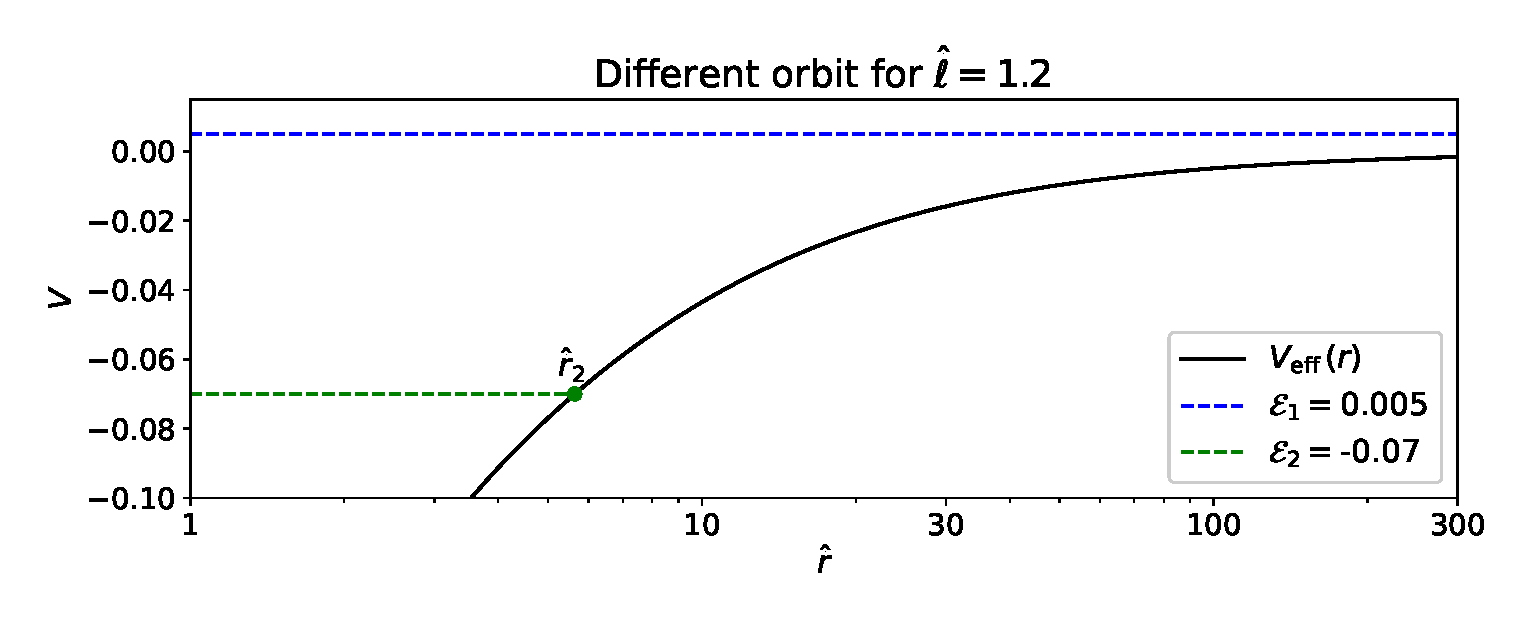
\includegraphics[width= 0.8 \textwidth]{Figures/chapter2/scenario0.eps}
    \caption{Possible scenarios for $\hat \ell < \sqrt{3}$.
    The outer turning points are labeled as $\hat r_2$ and the inner ones as}
    \label{cap2:fig:scenario0}
\end{figure}

\begin{figure}
    \centering
    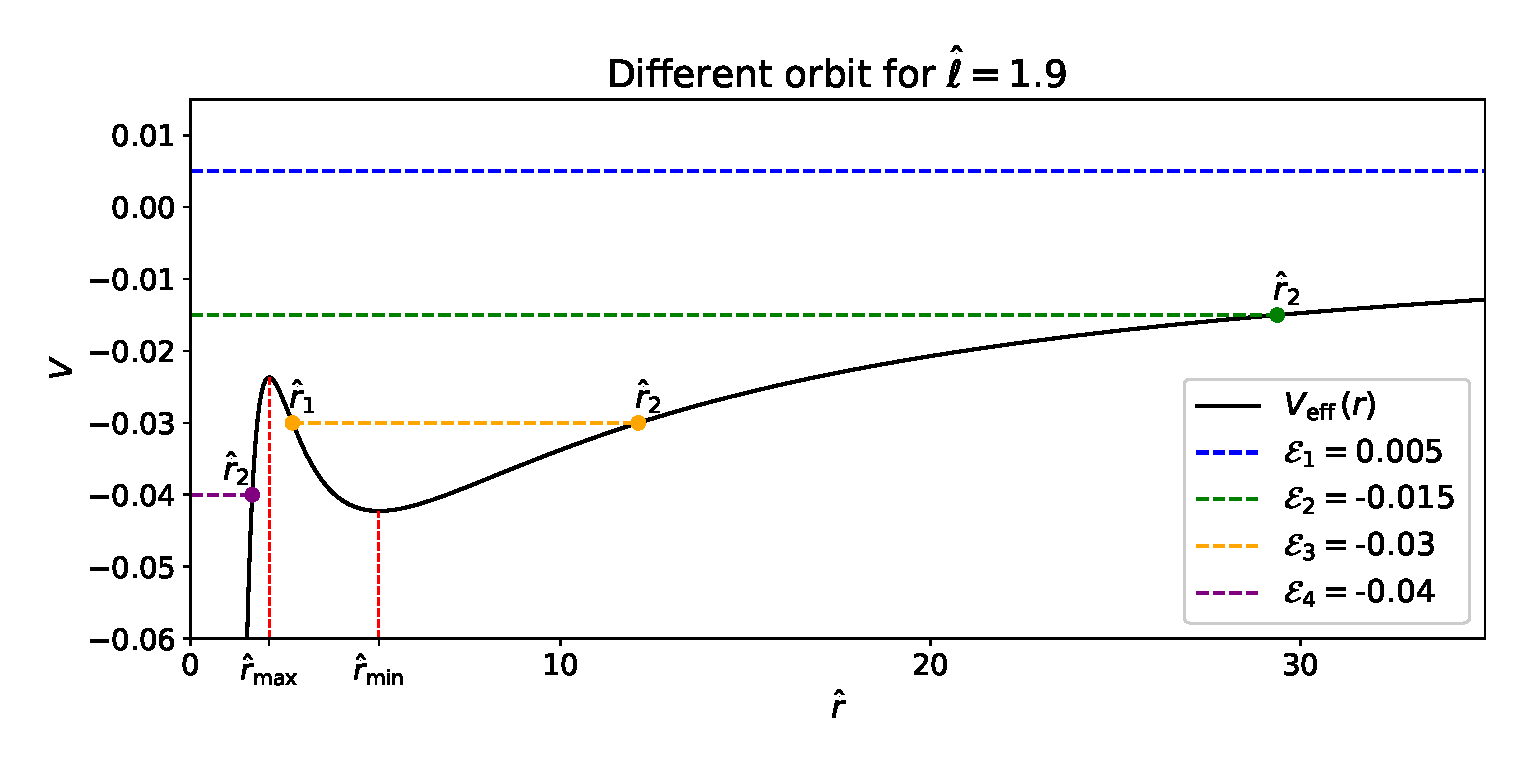
\includegraphics[width=\textwidth]{Figures/chapter2/scenario1.eps}
    \caption{Possible scenarios for $\hat \ell < 2$.
    The outer turning points are labeled as $\hat r_2$ and the inner ones as
    $\hat r_1$.
    Orbits with energy $\mathcal E > 0$ are infalls only if the minus sign is
    chosen in eq. \ref{cap2:eq:radial_eq_ad}.
    Orbits with energy like $\mathcal E_3$ can be bound orbits or infalls
    depending on the initial radius $\hat r_0$ chosen.
    Orbits like $\mathcal E_2$ are effectively infalls like $\mathcal E_4$, with
    the difference that the radial velocity of the particle will slow during
    between $r_{\rm min}$ and $r_{\rm max}$.}
    \label{cap2:fig:scenario1}
\end{figure}

\begin{figure}
    \centering
    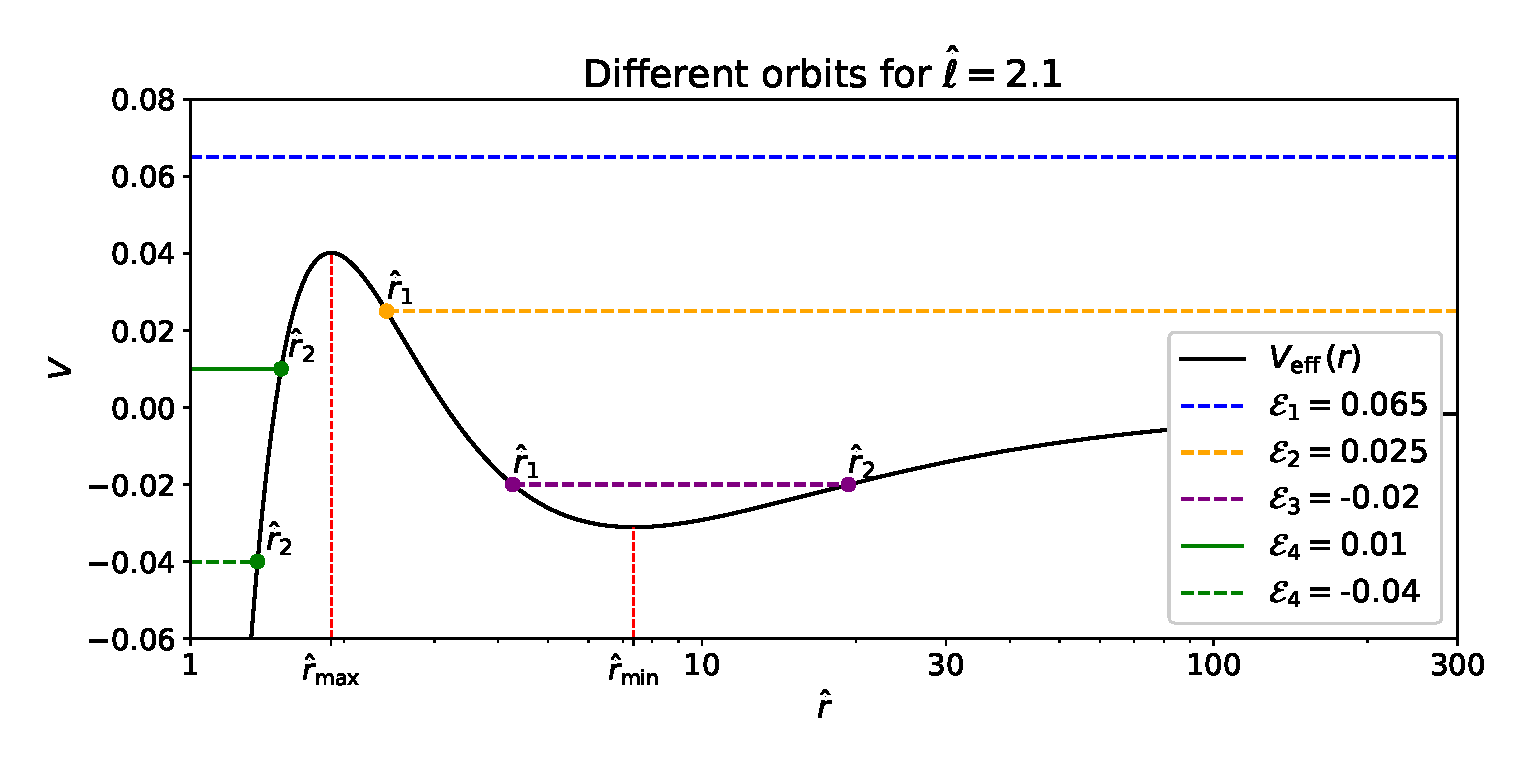
\includegraphics[width=\textwidth]{Figures/chapter2/scenario2.eps}
    \caption{Possible scenarios for $\hat \ell > 2$.
    The outer turning points are labeled as $\hat r_2$ and the inner ones as
    $\hat r_1$.
    Orbits with energy $\mathcal E > V_{\rm max}$ are infalls only if the minus
    sign is chosen in eq. \ref{cap2:eq:radial_eq_ad}.
    Orbits with $\mathcal E < V_{\rm max}$ can be infalls (purple) if the starting
    radius is small enough.
    Bound and unbound orbits are represented in yellow and green.}
    \label{cap2:fig:scenario2}
\end{figure}

The program can determine whether a turning point exists and can choose the correct
interval based on the initial conditions $ \hat{\ell} $ and $ \mathcal{E} $.
Fixing the limit of the numerical simulation at \texttt{R\_MAX = 1000}, when the
inner turning point $ \hat{r}_1 $ exists, it is always in the interval 
$[\hat{r}_{\text{max}}, ~ \hat{r}_{\text{min}}]$.
When the outer turning point $ \hat{r}_2 $ exists, it is always in the interval 
$[1, ~ \hat{r}_{\text{max}}]$ or $[\hat{r}_{\text{min}}, ~ \texttt{R\_MAX}]$.
This allows the program to check if the starting radius $ \hat{r}_0 $ is in an
allowed interval and, if not, to move it to the closest turning point, from
where the particle will start its motion.

All the possible scenarios are summarized in Table \ref{cap2:tab:scenarios}.

%\begin{table}[h]
%    \centering
%    \begin{tabular}{cccc}
%        \toprule
%        $\hat \ell$     & $\mathcal E$                              & $\hat r$                    & Scenario \\
%        \midrule
%        $[0,~\sqrt{3}]$ & $\left[0,~\infty \right)$            & $\left(1,~  \infty \right)$ & depends on the sign\\
%        $[0,~\sqrt{3}]$ & $\left[-\infty,~0 \right)$           & $\left(1,~     r_2 \right)$ & infall \\
%        $(\sqrt{3},~2]$ & $\left[0,~\infty \right)$            & $\left(1,~  \infty \right)$ & depends on the sign \\
%        $(\sqrt{3},~2]$ & $\left[V_{\rm max},~0 \right]$            & $\left(1,~     r_2 \right)$ & infall \\
%        $(\sqrt{3},~2]$ & $\left[V_{\rm min},~V_{\rm max} \right]$  & $\left(r_1,~   r_2 \right)$ & bound orbit \\
%        $(\sqrt{3},~2]$ & $\left[-\infty,~V_{\rm min} \right]$ & $\left(1,~     r_2 \right)$ & infall \\
%        $(2, \infty)$   & $\left[V_{\rm max},~\infty \right)$  & $\left(1,~  \infty \right)$ & depends on the sign \\
%        $(2, \infty)$   & $\left[0,~V_{\rm max} \right]$            & $\left(r_1,~\infty \right)$ & unbound orbit \\
%        $(2, \infty)$   & $\left[V_{\rm min},~V_{\rm min} \right]$  & $\left(r_1,~   r_2 \right)$ & bound orbit \\
%        $(2, \infty)$   & $\left[-\infty,~V_{\rm min} \right]$ & $\left(1,~     r_2 \right)$ & infall \\
%        \bottomrule
%    \end{tabular}
%    \caption{Possible scenarios for the motion of a particle in the \Sh
%    spacetime.}
%    \label{cap2:tab:scenarios}
%\end{table}

%% Dubbio valori di massimi e minimi di E

\begin{table}[h]
    \centering
    \begin{tabular}{c@{\hspace{1cm}}r@{}c@{}c@{}c@{}l@{\hspace{1cm}}c@{\hspace{1cm}}c}
        \toprule
        $\hat \ell$     &    &&$\mathcal E$      &             &    & $\hat r_0$                  & Scenario            \\
        \midrule
        $[0,~\sqrt{3}]$ & $[$&$0            $&$,$&$\infty     $&$)$ & $\left(1,~  \infty \right)$ & depends on the sign \\[0.1cm]
        $[0,~\sqrt{3}]$ & $($&$-\frac{1}{2} $&$,$&$0          $&$)$ & $\left(1,~     r_e \right)$ & infall              \\[0.1cm]
        $(\sqrt{3},~2]$ & $[$&$0            $&$,$&$\infty     $&$)$ & $\left(1,~  \infty \right)$ & depends on the sign \\[0.1cm]
        $(\sqrt{3},~2]$ & $[$&$V_{\rm max}  $&$,$&$0          $&$]$ & $\left(1,~     r_2 \right)$ & infall              \\[0.1cm]
        $(\sqrt{3},~2]$ & $[$&$V_{\rm min}  $&$,$&$V_{\rm max}$&$]$ & $\left(r_1,~   r_2 \right)$ & bound orbit         \\[0.1cm]
        $(\sqrt{3},~2]$ & $($&$-\frac{1}{2} $&$,$&$V_{\rm min}$&$]$ & $\left(1,~     r_e \right)$ & infall              \\[0.1cm]
        $(2, \infty)$   & $[$&$V_{\rm max}  $&$,$&$\infty     $&$)$ & $\left(1,~  \infty \right)$ & depends on the sign \\[0.1cm]
        $(2, \infty)$   & $[$&$0            $&$,$&$V_{\rm max}$&$]$ & $\left(r_1,~\infty \right)$ & unbound orbit       \\[0.1cm]
        $(2, \infty)$   & $[$&$V_{\rm min}  $&$,$&$V_{\rm min}$&$]$ & $\left(r_1,~   r_2 \right)$ & bound orbit         \\[0.1cm]
        $(2, \infty)$   & $($&$-\frac{1}{2} $&$,$&$V_{\rm min}$&$]$ & $\left(1,~     r_e \right)$ & infall              \\
        \bottomrule
    \end{tabular}
    \caption{Possible scenarios for the motion of a particle in the Schwarzschild spacetime.}
    \label{cap2:tab:scenarios}
\end{table}


One last detail to consider is the change of sign in eq.
\ref{cap2:eq:radial_eq_ad}.
To allow the particle to change radial direction an int \texttt{sign} that has
value $+1$ or $-1$ is passed to the function corresponding to the radial
derivative.
The code snippet is shown in Listing \ref{cap2:lst:sign_change} below.

\begin{lstlisting}[language=C, label=cap2:lst:sign_change, caption=Function to compute the radial derivative]
double TESI_fun_r(double r, double E, double l, int *sign, int *Nturns){
    double foo = 2 * (E - TESI_Veff(r, l));
    if (foo < 0){
        *sign *= -1;
        *Nturns += 1;
    }
    return *sign * pow(fabs(foo), 1. / 2.);
}
\end{lstlisting}

\texttt{E} is $\mathcal E$, \texttt{l} is $\hat \ell$ and \texttt{TESI\_Veff()} is
the function that computes the effective potential.
If \texttt{foo} is negative, the sign is changed and the number of turns
updated.
Then the square root is computed with the correct sign and taking the absolute
value of \texttt{foo}.
This is a simple way of handling the particle getting close and crossing the
turning point, but adds a small error in the overall computation of the other
variables as we allow the particle to overshoot the turning point.
At the beginning of the simulation we will always set
$\hat \tau = \hat \phi = \hat t = 0$ and, unless otherwise specified, the step
increment performed on $\hat \tau$ for each iteration of \texttt{RK4} will be
$h = 0.001$.

\newpage


\section{Infalls}

Similarly to the previous chapter, we can start with a radial infall scenario,
where $\hat \ell = 0$, $\mathcal E = 0$.

\begin{figure}[h]
    \begin{minipage}{0.48\textwidth}
        \centering
        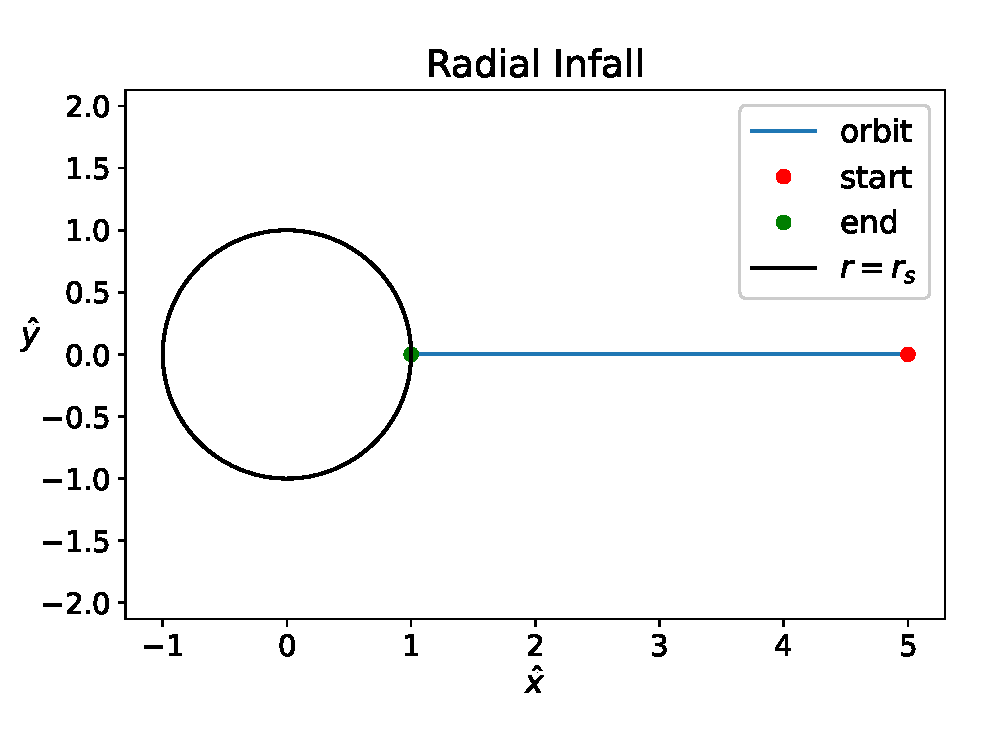
\includegraphics[width=\textwidth]{Figures/chapter2/radial_infall.eps}
        \caption{Plot of the orbit of a particle in radial infall
        ($\hat \ell = 0$, $\mathcal E = 0$, $r_0 = 5$, $h = 10^{-4}$). \\}
        \label{cap2:fig:radial_infall}
    \end{minipage}
    \hspace{0.015 \textwidth}
    \begin{minipage}{0.48\textwidth}
        \centering
        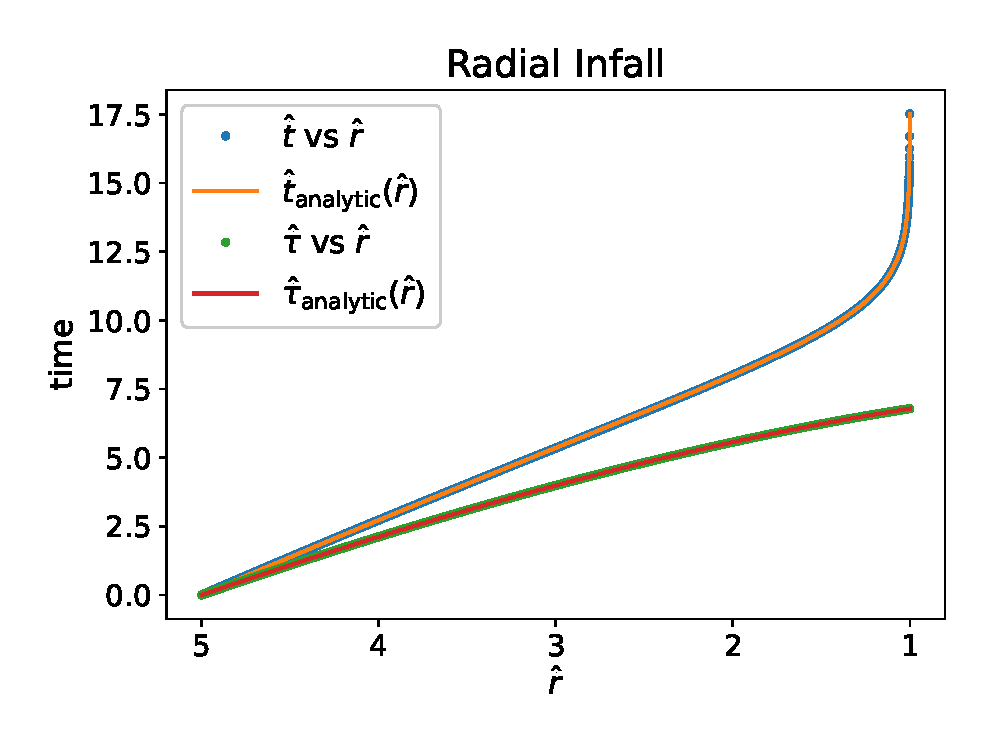
\includegraphics[width=\textwidth]{Figures/chapter2/t_vs_tau.eps}
        \caption{Proper time against \Sh time with respect of the radius of a
        particle falling towards $r = r_s$.
        (Data from Figure \ref{cap2:fig:radial_infall}).}
        \label{cap2:fig:t_vs_tau}
    \end{minipage}
\end{figure}

The orbit plot (Figure \ref{cap2:fig:radial_infall}) is not the most
interesting, but the time plot (Figure \ref{cap2:fig:t_vs_tau}) shows that the
numerical integration is working correctly, as the results are consistent with
eq. \ref{cap1:eq:radial_infall_r_of_tau} and \ref{cap1:eq:radial_infall_r_of_t}
found analytically in the previous chapter. \\
Figures \ref{cap2:fig:t_res} and \ref{cap2:fig:tau_res} also show the residuals
of $\hat t$ and $\hat \tau$ with respect to their analytical predictions.
For $\hat \tau$ the error is of the order of $10^{-10}$.
For $\hat t$ the vertical axis is in logarithmic scale to show that the error is
constant around $10^{-10}$, only to increase when the particle gets closer to
the \Sh radius.
That's to be expected as $t \rightarrow \infty$ when $r \rightarrow r_s$.

\begin{figure}[h]
    \begin{minipage}{0.48\textwidth}
        \centering
        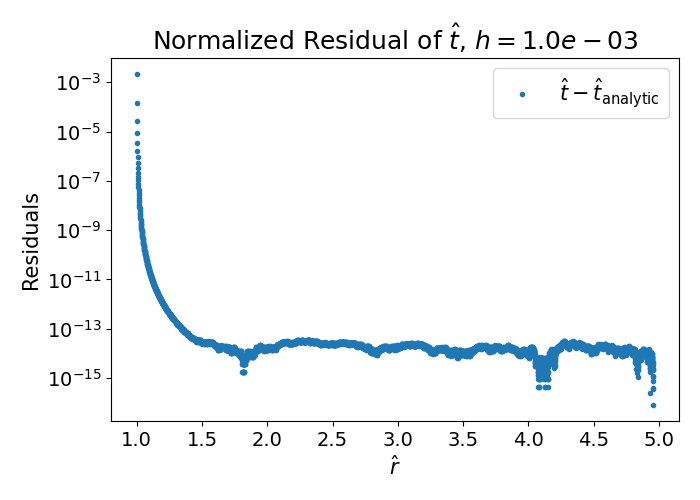
\includegraphics[width=\textwidth]{Figures/chapter2/t_res.png}
        \caption{Residual plot of $\hat t$ against the analytical prediction
        found in eq. \ref{cap1:eq:radial_infall_r_of_t}. \\
        (Data from Figure \ref{cap2:fig:radial_infall})}
        \label{cap2:fig:t_res}
    \end{minipage}
    \hspace{0.015 \textwidth}
    \begin{minipage}{0.48\textwidth}
        \centering
        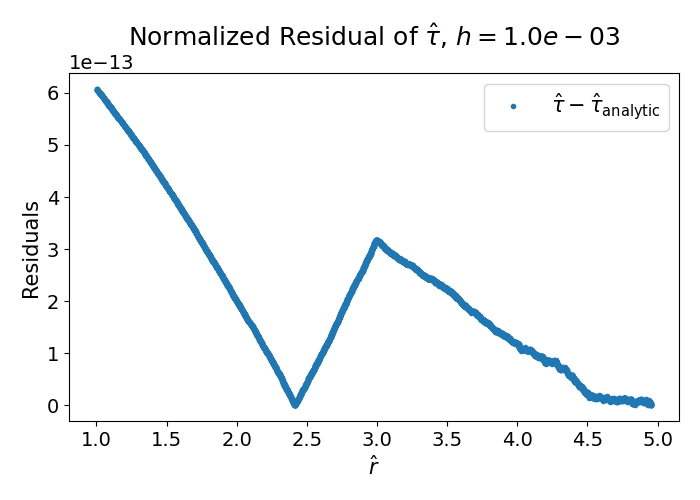
\includegraphics[width=\textwidth]{Figures/chapter2/tau_res.png}
        \caption{Residual plot of $\hat \tau$ against the analytical prediction
        found in eq. \ref{cap1:eq:radial_infall_r_of_tau}. \\
        (Data from Figure \ref{cap2:fig:radial_infall})}
        \label{cap2:fig:tau_res}
    \end{minipage}
\end{figure}

By integrating numerically with this program, we can visualize some more
complex infalls that are shown in Figures \ref{cap2:fig:infall1} and
\ref{cap2:fig:infall2}.

\begin{figure}[h]
    \begin{minipage}{0.48\textwidth}
        \centering
        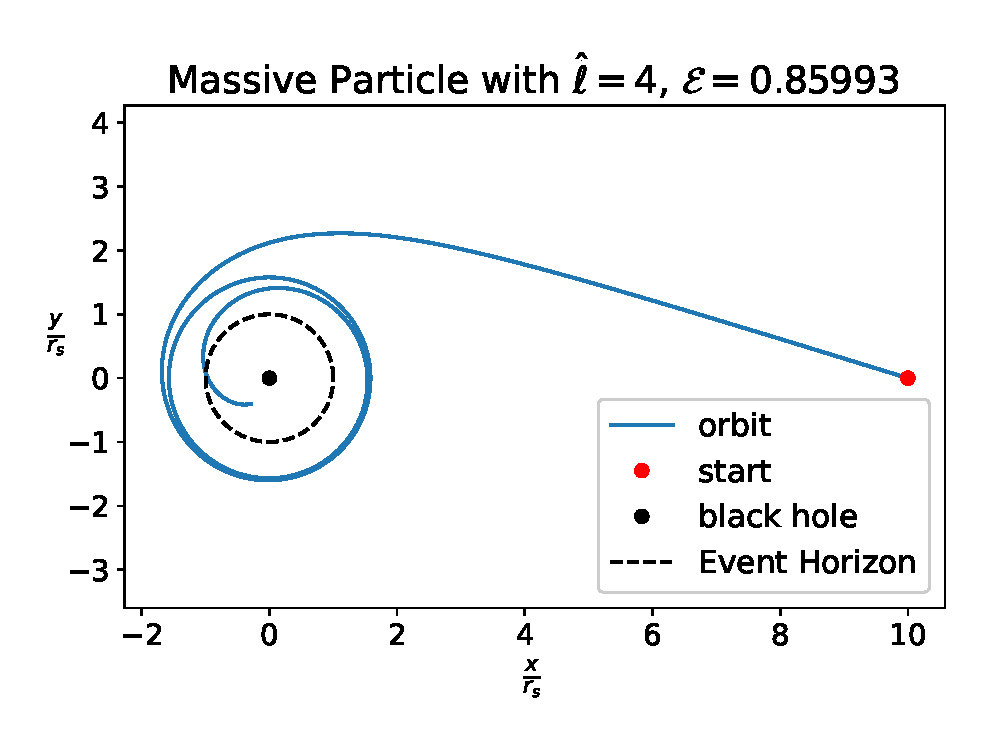
\includegraphics[width=\textwidth]{Figures/chapter2/infall1.eps}
        \caption{The particle starts at $\hat r_0 = 10$
        ($\hat r_{\rm max} \simeq 1.6$) and has an energy slightly greater than
        $V_{\rm eff}(r_{\rm max}) \simeq 0.859927$.
        As a result the radial velocity decreases when the particle passes
        through $\hat r = \hat r_{\rm max}$.}
        \label{cap2:fig:infall1}
    \end{minipage}
    \hspace{0.015 \textwidth}
    \begin{minipage}{0.48\textwidth}
        \centering
        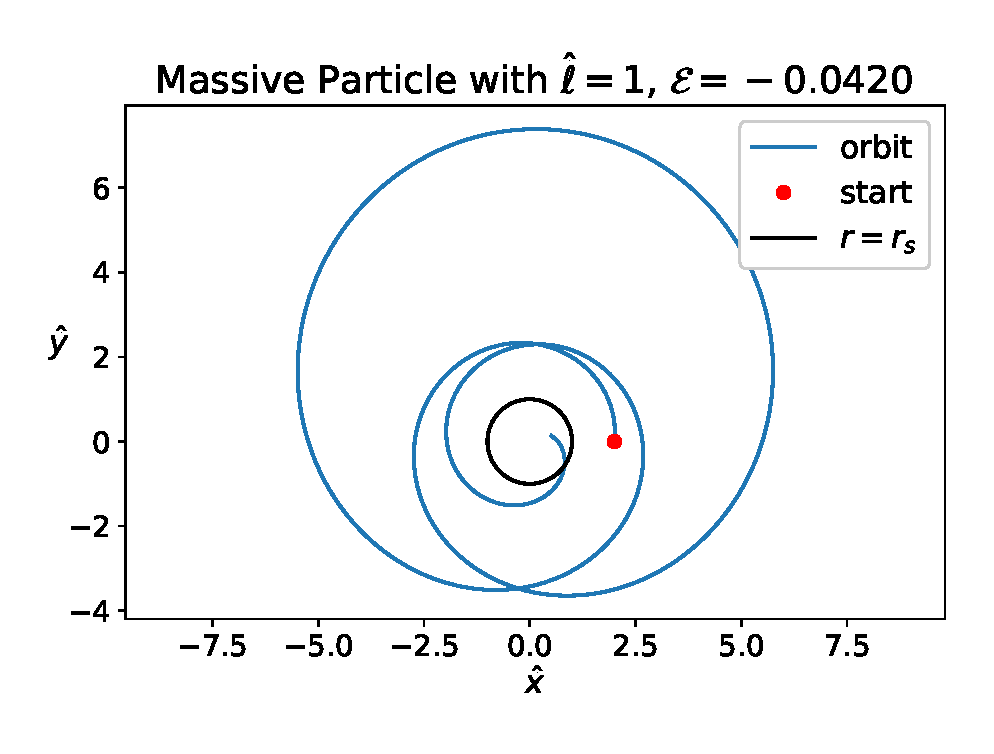
\includegraphics[width=\textwidth]{Figures/chapter2/infall2.eps}
        \caption{$V_{\rm eff}$ is monotonic because $\ell < \sqrt{3}$.
        The particle starts at $\hat r = 2$ with its radial velocity
        directed outward; however, due to its negative energy $\mathcal E$, the
        particle will not be able to escape.}
        \label{cap2:fig:infall2}
    \end{minipage}
\end{figure}

\begin{figure}[h!]
    \centering
    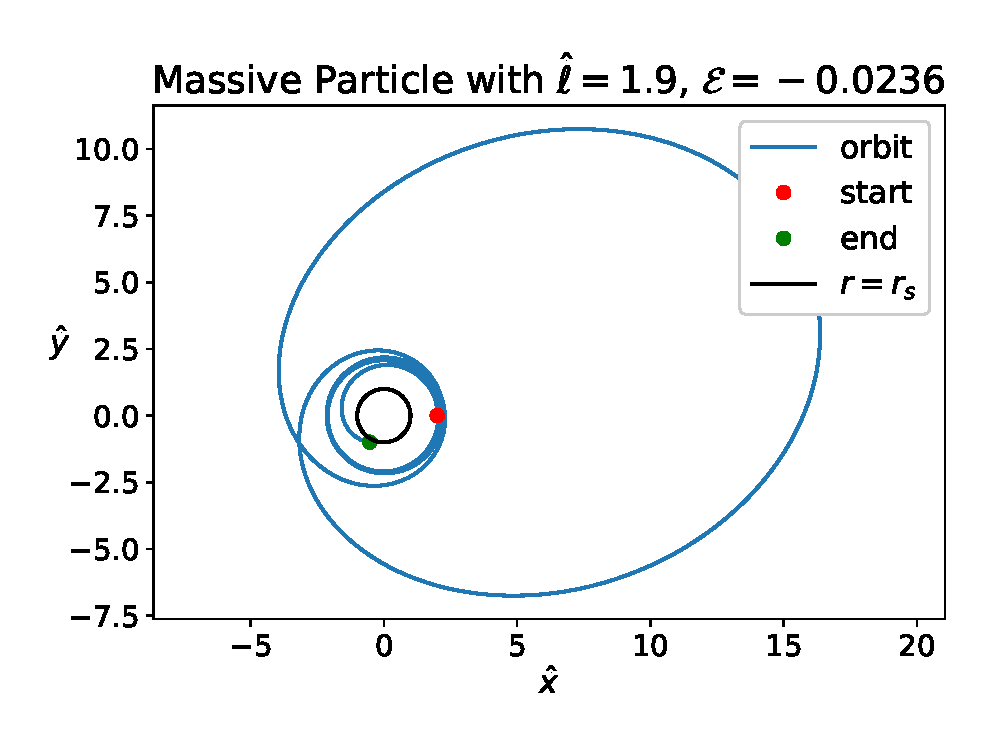
\includegraphics[width=0.73 \textwidth]{Figures/chapter2/volevi.eps}
    \caption{The particle starts at $\hat r_0 = 2$ with $\hat \ell = 1$,
    $\mathcal E = -0.02367591$ and its radial velocity directed outward.
    $V_{\rm eff} (\hat r_{\rm max} = 2.13) = -0.02367592$, meaning the particle
    has just enough energy to surpass the potential barrier.
    However, the radial velocity will almost go to zero at
    $\hat r \simeq \hat r_{\rm max}$.
    This results in the particle almost starting a circular orbit, completing
    three full revolutions before gradually moving farther from the origin
    The radial velocity then increases unit
    $\hat r > \hat r_{\rm min} \simeq 5$, where the potential rises again.
    The energy is sufficient to reach the turning point at $r_2 \simeq 16.9$,
    after which the particle falls back toward the origin, performing three more
    turns around $\hat r \simeq 2.13$.}
    \label{cap2:fig:volevi}
\end{figure}


\section{Bound Orbits}

To study bound orbits we need to consider particles with $\hat \ell > \sqrt{3}$
and $V_{\rm min} \leq \mathcal E < \min \{V_{\rm max}, 0\}$.

\subsection{Circular Orbits}

As seen in section \ref{cap1:ssec:circular_orbits} in the previous chapter we
have a circular orbit only if $\mathcal E = V_{\rm min}$.
In this case the relation found in eq. \ref{cap1:eq:Omega2} holds:

\begin{equation}
    \hat \Omega^2 = \frac{1}{2 \hat r^3}
    \quad \quad \quad {\rm where} \quad \quad \quad
    \hat \Omega := \dv{\phi}{\hat t} \, .
    \label{cap2:eq:Omega2}
\end{equation}

In Figure \ref{cap2:fig:circ_orbit} we can see the orbit of a particle with
$\hat \ell = 3$ and $\mathcal E = V_{\rm min} \simeq
\num{-1.478e-02}$.
Figure \ref{cap2:fig:circ_orbit_res} shows the normalized residuals of the
angular velocity $\hat \Omega$ computed from $\phi$ and $\hat t$ obtained
during the simulation against the expected value evaluated from eq.
\ref{cap2:eq:Omega2} with the initial radius $\hat r_{\rm min}$.

\begin{figure}[h]
    \begin{minipage}{0.48\textwidth}
        \centering
        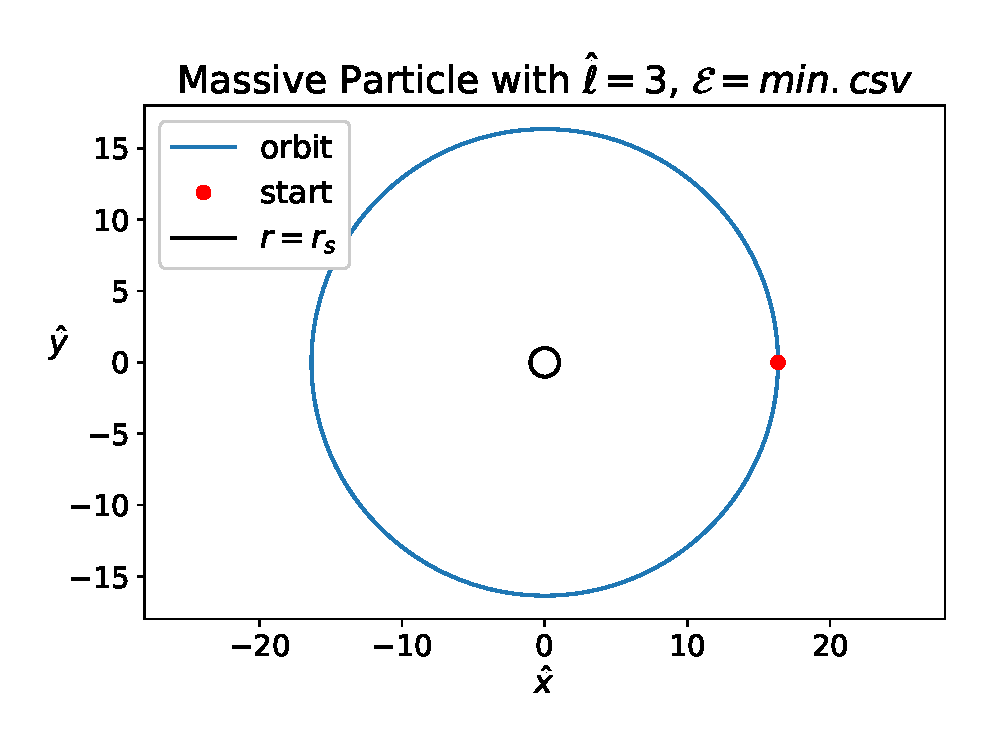
\includegraphics[width=\textwidth]{Figures/chapter2/circ.eps}
        \caption{The perfectly circular orbit of a particle ($\hat \ell = 3$,
        $\mathcal E = V_{\rm min} \simeq \num{-1.478e-02}$).
        The particle starts at $\hat r = r_{\rm min} \simeq 16.35$ and the
        radius is left unchanged.}
        \label{cap2:fig:circ_orbit}
    \end{minipage}
    \hspace{0.015 \textwidth}
    \begin{minipage}{0.48\textwidth}
        \centering
        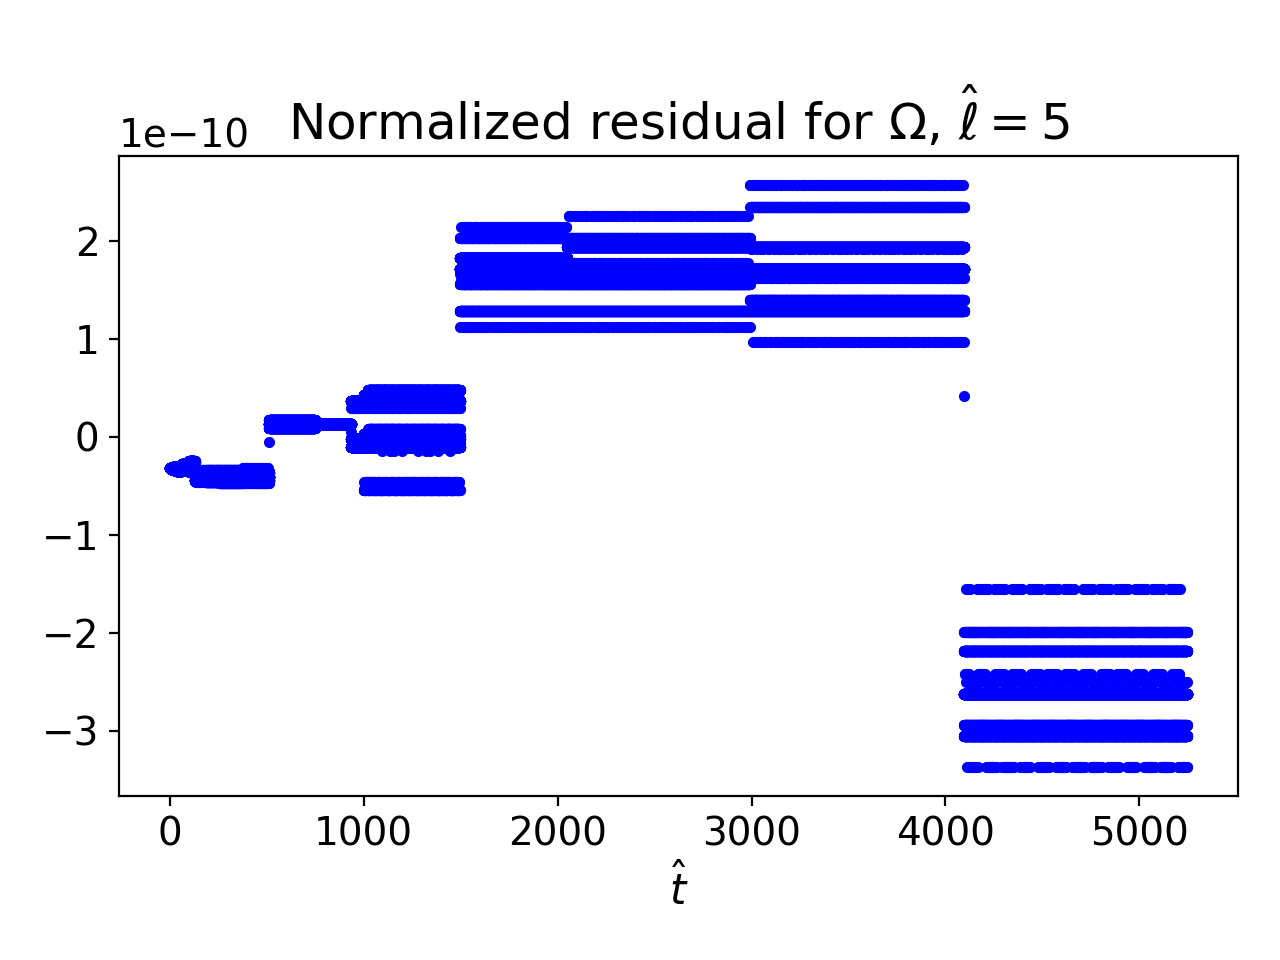
\includegraphics[width=1.08\textwidth]{Figures/chapter2/circ_res.png}
        \caption{The residual of the angular velocity $\hat \Omega$ computed
        from the data of $\phi$ and $\hat t$ with respect to the expected value 
        $\hat \Omega_{\rm analytic}
        = 1 / (2 ~ \hat r_{\rm min}) \simeq \num{1.07e-2}$.}
        \label{cap2:fig:circ_orbit_res}
    \end{minipage}
\end{figure}

The relative error is of order $10^{-10}$ with a time increment $h = 0.001$, we
can conclude that the numerical integration is correctly implemented and most
of the error comes from the finite precision.

Therefore, we can proceed with confidence to study bound orbits of different
shapes.


\subsection{Precession}

Recall from eq. \ref{cap1:eq:precession} and \ref{cap1:eq:delta_phi} that, for a
bound orbit where the two turning points are, as usual, labeled $r_1 < r_2$, the
precession is given by

\begin{equation}
    \delta \phi = 2 \int_{r_1}^{r_2} \left( 2 \mathcal E + \frac{2M}{r}
    - \frac{l^2}{r^2} + \frac{2Ml^2}{r^3} \right)^{-1/2} \, \dd{r}
    \; - 2 \pi \, .
\end{equation}

If we make the substitution $r = 1 / u$ and use the definition of $\mathcal E
= \frac{e^2 - 1}{2}$, we can rewrite the integral as

\begin{equation}
    \delta \phi = 2 \int_{u_2}^{u_3} \frac{1}{\sqrt{2 \mathcal E + 2Mu - l^2 u^2
    + 2Ml^2 u^3}} \, \dd{u}
    \; - 2 \pi \, .
    \label{cap2:eq:delta_phi}
\end{equation}

The bounds of the integral are $u_2 = 1 / r_2 < u_3 = 1 / r_1$.
Under the square root we have a cubic equation in $u$ with

\begin{align}
    &{\rm coefficients} && a = 2Ml^2, \quad b = -l^2, \quad c = 2M, \quad d = 2 \mathcal E \\
    &{\rm roots}        && u_1, ~ u_2, ~ u_3 \, .
    \label{cap2:eq:cubic_roots}
\end{align}

Since all the coefficients are real, the roots of the equation must either
consist of three real numbers or one real root and a pair of complex conjugate
roots.
Given that we are considering bound orbits, we know that two real roots must
exist.
Therefore, we can infer that all three roots are real and can be labeled such
that $u_1 < u_2 < u_3$.

The Wikipedia article \textit{Precession of orbits} \footcite{enwiki:1242536958}
shows that, knowing the roots in \ref{cap2:eq:cubic_roots}, the integral in
\ref{cap2:eq:delta_phi} can be expressed in terms of the complete elliptic
integral of the first kind $K(m)$

\begin{equation}
    \delta \phi = 2 \int_{u_2}^{u_3} \frac{1}{\sqrt{(u - u_1)(u - u_2)(u - u_3)}}
    \, \dd{u} \; - 2 \pi
    = \frac{K(m)}{\sqrt{r_s (u_3 - u_1)}} - 2 \pi \, .
    \label{cap2:eq:delta_phi_elliptic}
\end{equation}

Where $K$ and $m$ are respectively defined as

\begin{equation}
    K(m) = \int_0^{\pi/2} \frac{\dd{\theta}}{\sqrt{1 - m \sin^2 \theta}} \, ,
    \quad \quad \quad
    m = \frac{u_2 - u_1}{u_3 - u_1}
\end{equation}

and can be numerically solved in python using the \texttt{scipy.special.ellipk}
function.

We can now compare the precession of a particle computed from the numerical data
of the simulation with the expected value calculated from the initial conditions
with the library for elliptic integrals.

Figure \ref{cap2:fig:prec1} \ref{cap2:fig:prec2} shows two examples of bound
orbits with different values of $\hat \ell$ and $\mathcal E$, giving rise to
different precessions.

\begin{figure}[h]
    \begin{minipage}{0.48 \textwidth}
        \centering
        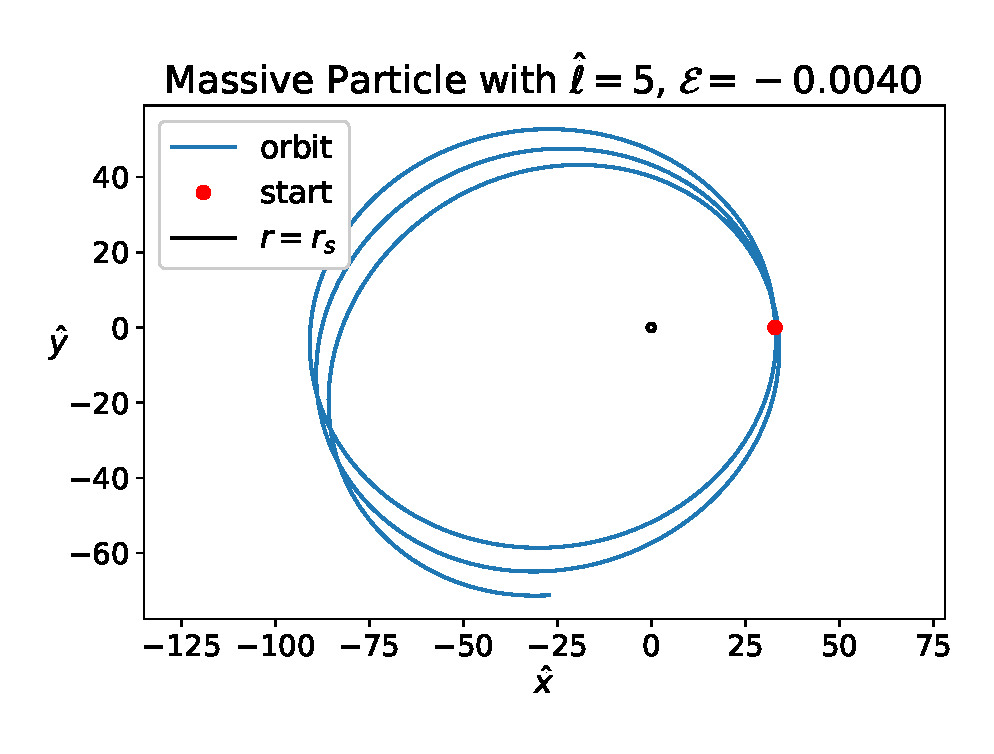
\includegraphics[width=\textwidth]{Figures/chapter2/prec1.eps}
        \caption{$\hat \ell = 5$, $\mathcal E = -0.004$,
        $\hat r_0 = r_1 \simeq 32.9$, evolved for $\hat \tau = \num{1.2e5}$. \\
        $\delta \phi_{\rm theory} \simeq 0.0652 \pi$ from eq.
        \ref{cap2:eq:delta_phi_elliptic}.}
        \label{cap2:fig:prec1}
    \end{minipage}
    \hspace{0.015 \textwidth}
    \begin{minipage}{0.48 \textwidth}
        \centering
        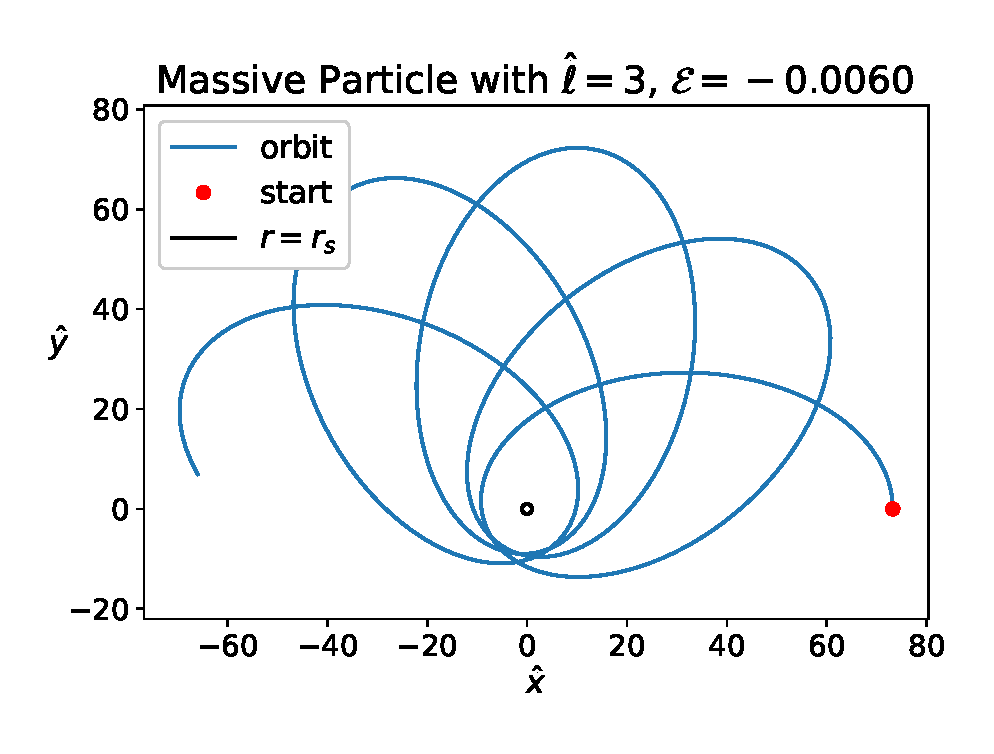
\includegraphics[width=\textwidth]{Figures/chapter2/prec2.eps}
        \caption{$\hat \ell = 3$, $\mathcal E = -0.006$,
        $\hat r_0 = r_1 \simeq 73.2$, evolved for $\hat \tau = \num{1e4}$. \\
        $\delta \phi_{\rm theory} \simeq 0.221 \pi$ from eq.
        \ref{cap2:eq:delta_phi_elliptic}.}
        \label{cap2:fig:prec2}
    \end{minipage}
\end{figure}

Letting the system evolve for a longer time, we can collect more data points.
The angle spanned by the particle in the $\phi$ direction can be computed from
the data of the simulation by looking at the angle corresponding to the local
maxima and minima of the radius.
Figure \ref{cap2:fig:prec1_res} and \ref{cap2:fig:prec2_res} show the residuals
of the precession angle computed from the simulation data with respect to the
expected value calculated from the initial conditions
(eq. \ref{cap2:eq:delta_phi_elliptic}).

\begin{figure}[h]
    \begin{minipage}{0.48 \textwidth}
        \centering
        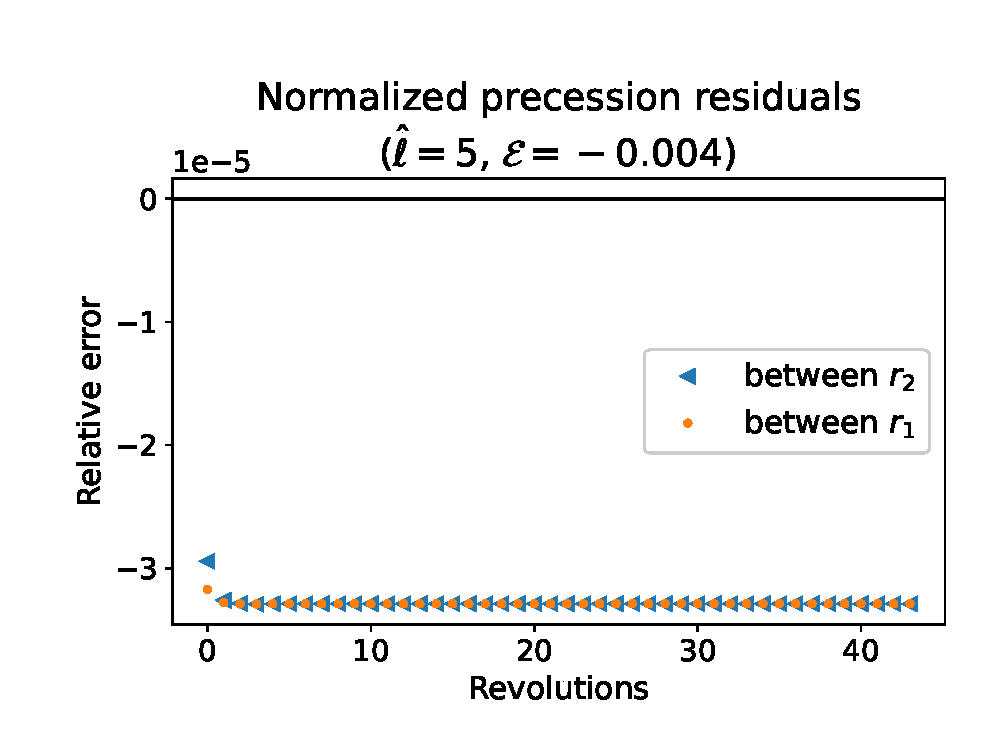
\includegraphics[width=\textwidth]{Figures/chapter2/prec1_res.eps}
        \caption{The simulation was run for $\hat \tau = \num{2e5}$.
        The expected precession angle is $\delta \phi_{\rm theory} \simeq 0.0652
        \pi$.
        The relative error is quite small, in the order of $10^{-5}$, but we are
        systematically underestimating the precession.
        Averaging the $\delta \phi$ values obtained from $\hat r_2$ we get: \\
        $\delta \phi_{\rm avg} = \delta \phi_{\rm theory} - \num{7e-6} \pm \num{2e-8}$.}
        \label{cap2:fig:prec1_res}
    \end{minipage}
    \hspace{0.015 \textwidth}
    \begin{minipage}{0.48 \textwidth}
        \centering
        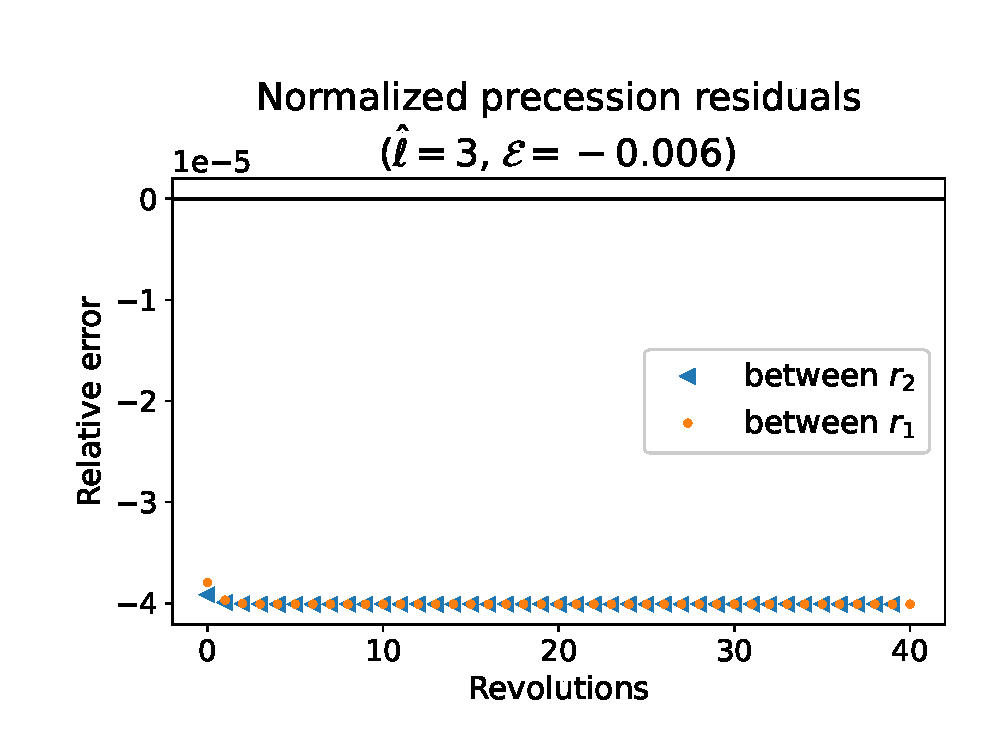
\includegraphics[width=\textwidth]{Figures/chapter2/prec2_res.eps}
        \caption{The simulation was run for $\hat \tau = \num{1e5}$.
        The expected precession angle is $\delta \phi_{\rm theory} \simeq 0.221
        \pi$.
        The relative error is quite small, in the order of $10^{-5}$, but we are
        systematically underestimating the precession.
        Averaging the $\delta \phi$ values obtained from $\hat r_2$ we get: \\
        $\delta \phi_{\rm avg} = \delta \phi_{\rm theory} - \num{3e-5} \pm \num{2e-8}$.}
        \label{cap2:fig:prec2_res}
    \end{minipage}
\end{figure}

With a time increment $h = 0.001$ the relative error is of order $10^{-5}$.
The error is not as small as in the previous cases, but the most concerning
aspect is that we are systematically underestimating the precession.
As mentioned when presenting the code snippet \ref{cap2:lst:sign_change} used to
evaluate the radial derivative, the particle is allowed to overshoot the turning
point.
In particular when the argument of the square root ($2 \mathcal E
- 2 V_{\rm eff}$) is negative we just take the absolute value, change the sign
outside the square root and use that to compute the radial derivative.
In reality, the particle should get close to the turning point, its radial
velocity should slowly approach zero and then start increasing again, but with
an opposite sign.

It's important to note that the error is not given by the overshoot in itself,
but by the fact that the particle velocity never goes to zero, or at least
doesn't get close enough to it.
In fact, even if we used an adaptive step size method, that allows to take the
particle exactly to the turning point, we would still be overestimating the
modulus of the particle radial velocity (and therefore underestimating the
precession) as the acceleration is not negligible when the radial velocity is
very small.
Moreover, reducing the systematic error by reducing the step size brings a lot
of risks of numerical instability because of the singularity at the turning
point: the moment that the radius is really closer to a turning point the radial
derivative goes to zero and radius will not change anymore.
An alternative method to avoid this problem is presented in the next section.


\section{Alternative Integration Method}

To avoid the singularity of the radial derivative at the turning points, we can
use the second derivative instead.
Using the acceleration is in fact safer as it never goes to zero and does not
have sign changes to worry about.
We can therefore rewrite the system of equations \ref{cap2:eq:eq_of_motion_ad}
as

\begin{subequations}
    \begin{align}[left = {\empheqlbrace}]
        &\dv{\hat v}{\hat \tau} = - \dv{V_{\rm eff}}{\hat r} 
        = \frac{\hat \ell^2}{\hat r^3} - \frac{1}{2 r^2}
        - \frac{3 \hat \ell^2}{2 \hat r^4} \label{cap2:eq:acc_eq_ad} \\
        &\dv{\hat r}{\hat \tau} = \hat v \\
        &\dv{\phi}{\hat \tau} = \frac{\hat \ell}{\hat r^2} \\
        &\dv{t}{\hat \tau} = \sqrt{2 \mathcal E + 1}
        \left(\frac{\hat r}{\hat r - 1}\right)
        \label{cap2:eq:t_ad_v2}
    \end{align}
    \label{cap2:eq:eq_of_motion_v2}
\end{subequations}

where we defined $\hat v = \dv{\hat r}{\hat \tau}$ as the radial velocity of the
particle and derived eq. \ref{cap2:eq:radial_eq_ad} that in this case is
equivalent to deriving the effective potential with respect to $\hat r$.

This solution allows for a more precise computation of the precession angle.
We infact repeated the simulations represented in Figures 
\ref{cap2:fig:prec1} and \ref{cap2:fig:prec2} integrating the system in 
\ref{cap2:eq:eq_of_motion_v2} and the results are shown in Figures
\ref{cap2:fig:prec1_res_corr} and \ref{cap2:fig:prec2_res_corr}, and eliminate
any additional sign changes or risks of the particle getting stuck at the
turning point.

\begin{figure}[h]
    \begin{minipage}{0.48 \textwidth}
        \centering
        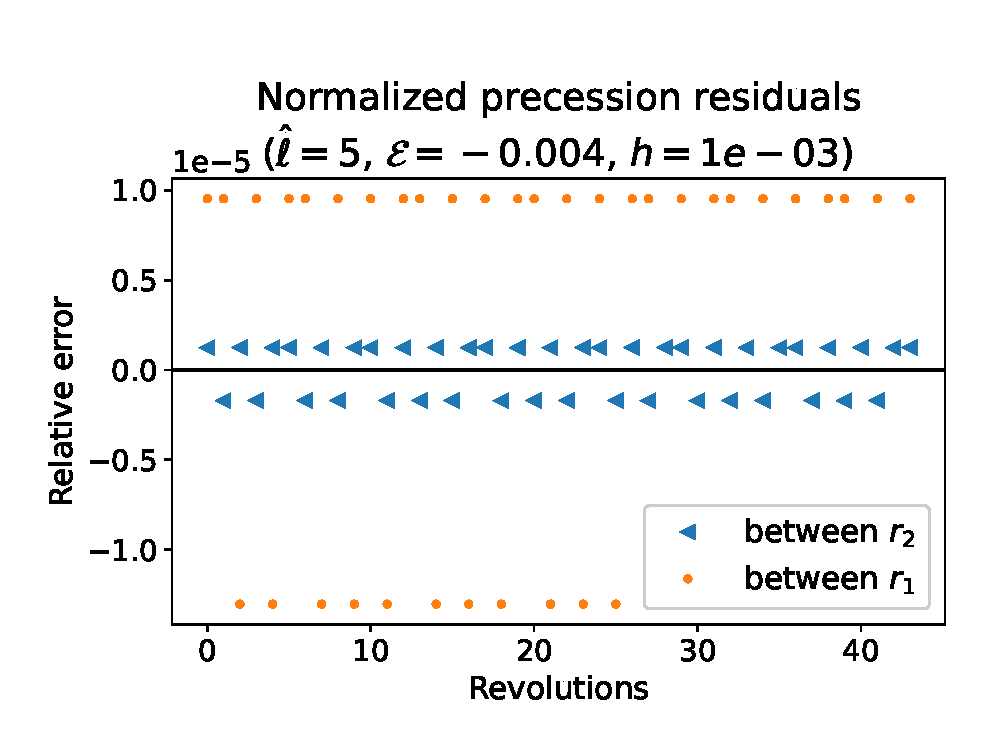
\includegraphics[width=\textwidth]{Figures/chapter2/prec1_res_corr.eps}
        \caption{The simulation was run for $\hat \tau = \num{2e5}$.
        The expected precession angle is $\delta \phi_{\rm theory} \simeq 0.0652
        \pi$.
        Averaging the $\delta \phi$ values obtained from $\hat r_2$ we get: \\
        $\delta \phi_{\rm avg} = \delta \phi_{\rm theory} + (8 \pm 40) \times \num{e-9}$.}
        \label{cap2:fig:prec1_res_corr}
    \end{minipage}
    \hspace{0.015 \textwidth}
    \begin{minipage}{0.48 \textwidth}
        \centering
        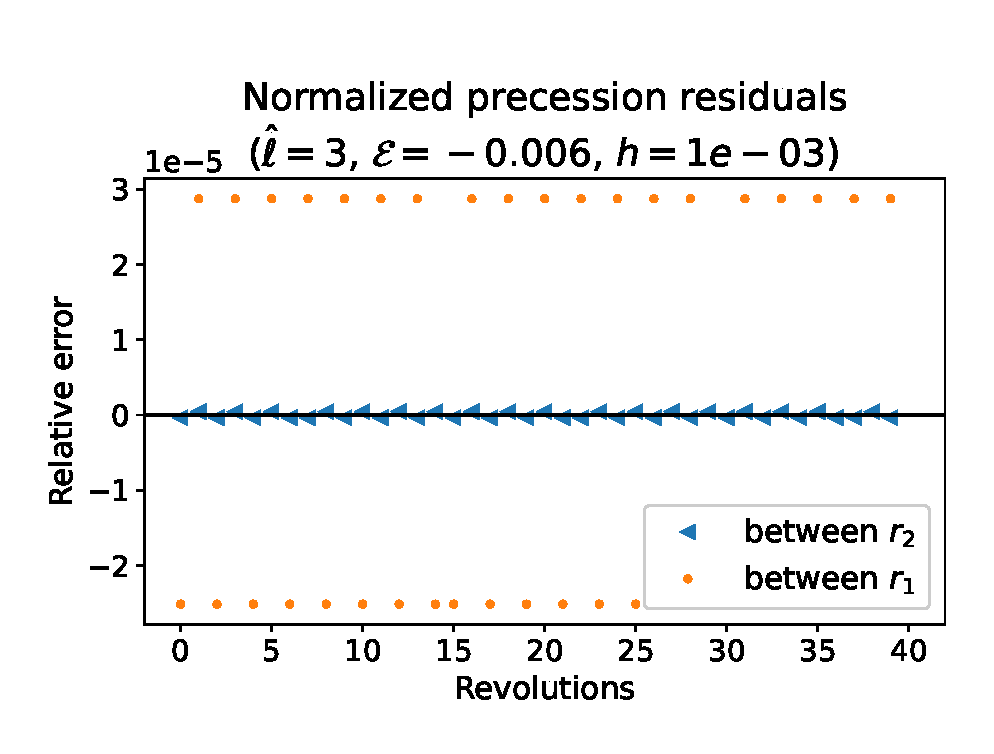
\includegraphics[width=\textwidth]{Figures/chapter2/prec2_res_corr.eps}
        \caption{The simulation was run for $\hat \tau = \num{1e5}$.
        The expected precession angle is $\delta \phi_{\rm theory} \simeq 0.221
        \pi$.
        Averaging the $\delta \phi$ values obtained from $\hat r_2$ we get: \\
        $\delta \phi_{\rm avg} = \delta \phi_{\rm theory} - (9 \pm 40) \times \num{e-9}$.}
        \label{cap2:fig:prec2_res_corr}
    \end{minipage}
\end{figure}

There are some drawbacks to this method, however.
The first one being the obvious increase in computational time, as we need
to simultaneously solve 4 differential equations with the \texttt{RK4} method
instead of 3.
The second one is that the energy of the particle $\mathcal E$ is not conserved
anymore: we in fact compute the velocity numerically, using the acceleration
in eq. \ref{cap2:eq:acc_eq_ad}, and not analytically from the $V_{\rm eff}$ and
$\mathcal E$ as in eq. \ref{cap2:eq:radial_eq_ad}.
This also makes it necessary to compute the energy ($\mathcal E = \hat v^2 / 2 +
V_{\rm eff}$) at each step of the simulation, before updating the \Sh time $t$ with eq. \ref{cap2:eq:t_ad_v2}. \\
For both the simulations run to compute the precession in Figure
\ref{cap2:fig:prec1_res_corr} and \ref{cap2:fig:prec2_res_corr} the energy 
relative error at the end is of order $10^{-13}$ (an energy loss to be precise),
negligible in this context, but it could be a problem for longer
simulations.

